\section{Difference Images} \label{sec:image_differences}

\begin{figure}[htb]
    \centering
        \begin{subfigure}[b]{0.42\textwidth}
            \centering
            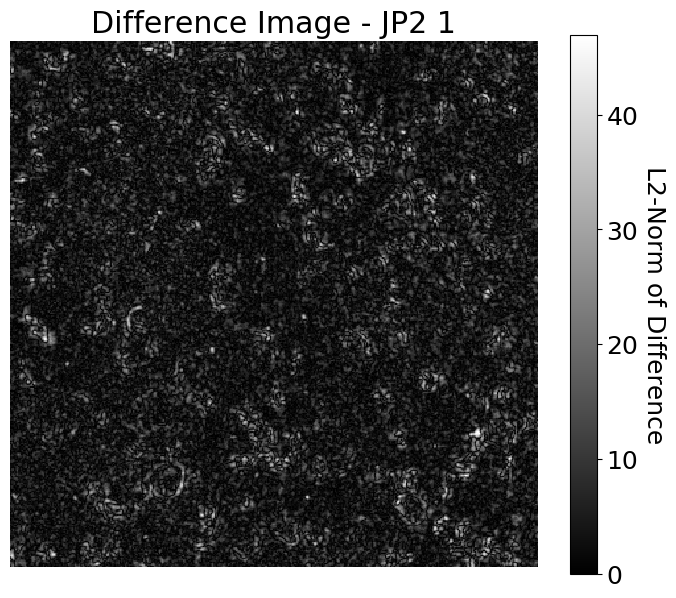
\includegraphics[width=\textwidth]{doc/thesis/0_figures/compare_quality/set1/jp2_1_center_diff_heatmap_rel.png}
            \caption{\gls{jp2} quality 1.}
            \label{fig:img_quality_center_heatmap_rel_1}
        \end{subfigure}
        \begin{subfigure}[b]{0.42\textwidth}
            \centering
            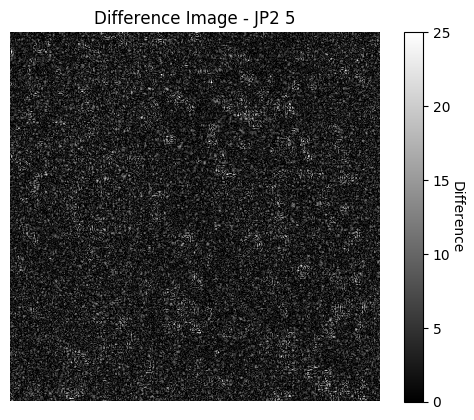
\includegraphics[width=\textwidth]{doc/thesis/0_figures/compare_quality/set1/jp2_5_center_diff_heatmap_rel.png}
            \caption{\gls{jp2} quality 5.}
            \label{fig:img_quality_center_heatmap_rel_5}
        \end{subfigure}
        \\
        \begin{subfigure}[b]{0.42\textwidth}
            \centering
            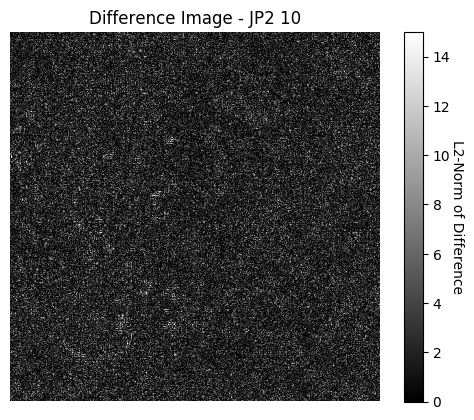
\includegraphics[width=\textwidth]{doc/thesis/0_figures/compare_quality/set1/jp2_10_center_diff_heatmap_rel.png}
            \caption{\gls{jp2} quality 10.}
            \label{fig:img_quality_center_heatmap_rel_10}
        \end{subfigure}
        \begin{subfigure}[b]{0.42\textwidth}
            \centering
            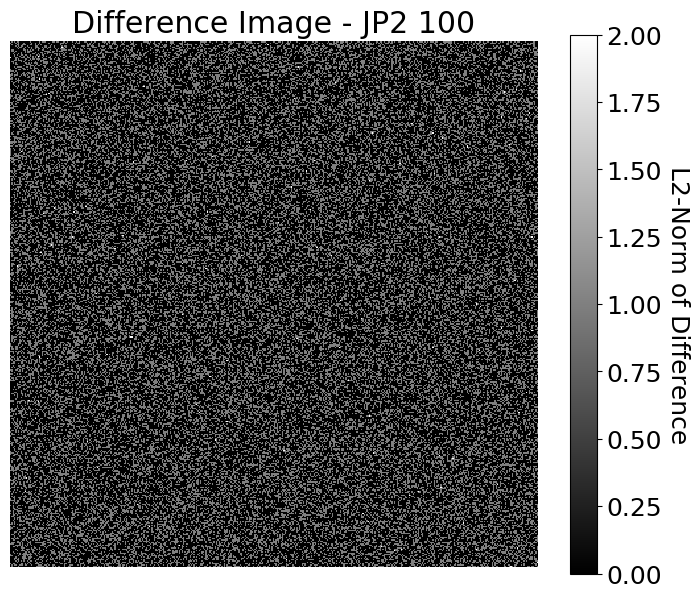
\includegraphics[width=\textwidth]{doc/thesis/0_figures/compare_quality/set1/jp2_100_center_diff_heatmap_rel.png}
            \caption{\gls{jp2} quality 100.}
            \label{fig:img_quality_center_heatmap_rel_100}
        \end{subfigure}
        \\
        \begin{subfigure}[b]{0.42\textwidth}
            \centering
            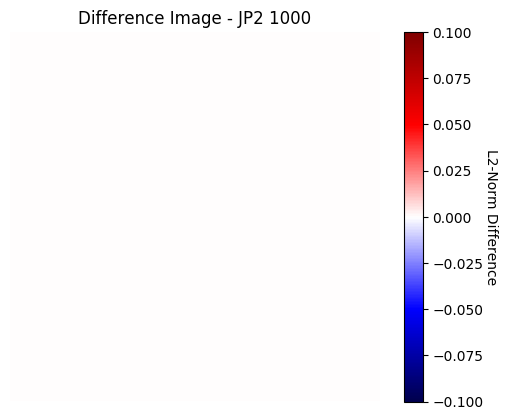
\includegraphics[width=\textwidth]{doc/thesis/0_figures/compare_quality/set1/jp2_1000_center_diff_heatmap_rel.png}
            \caption{\gls{jp2} quality 1000.}
            \label{fig:img_quality_center_heatmap_rel_1000}
        \end{subfigure}
        \begin{subfigure}[b]{0.42\textwidth}
            \centering
            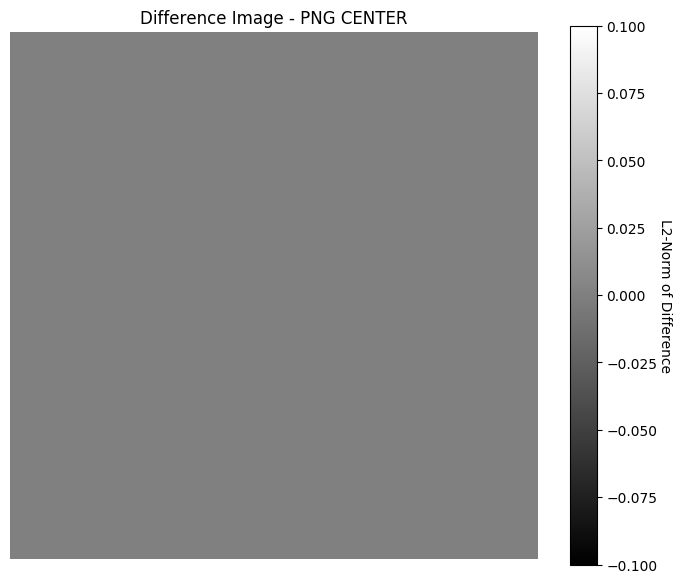
\includegraphics[width=\textwidth]{doc/thesis/0_figures/compare_quality/set1/png_center_diff_heatmap_rel.png}
            \caption{\gls{png}}
            \label{fig:img_quality_center_heatmap_rel_png}
        \end{subfigure}
    \caption{Difference images of close-ups with varying levels of compression using \gls{jp2} and one \gls{png} using different scales to show also smaller differences in the less compressed images. Image \ref{fig:img_quality_center_heatmap_rel_1000} is white because it does not differ from the \gls{png} image.}
    \label{fig:img_quality_center_heatmap_rel}
\end{figure}